% Chapter Template

\chapter{Implementation and experiment setup} % Main chapter title

\label{Chapter5} % Change X to a consecutive number; for referencing this chapter elsewhere, use \ref{ChapterX}
In this section we explain in detail, what hardware we used in our implementation and with which technology the UWB communication and ranging was done. Then we introduce the zone indication learning algorithm and finally we briefly explain the core of our work, the mathematical theory of the particle filter.

%----------------------------------------------------------------------------------------
%	SECTION 1
%----------------------------------------------------------------------------------------

\section{Hardware}
We decided to use Raspberry Pis for all mobile devices such as the TAG and the ANs. As the Raspberry Pis were not equipped with UWB technology, we extended them with a SEQUITUR Pi board from UNISET company running InGPS Lite firmware. In the following two subsections we present you these two hardware components.

%-----------------------------------
%	SUBSECTION 1
%-----------------------------------

\subsection{Raspberry Pi}
A Raspberry Pi is a single-board computer not much bigger than a credit card. Raspberry Pis are mainly designed for educational purposes as an alternative to expensive notebooks or desk computers. Hence the focus lies also on easy-to-use and plug-and-play experiences. Raspberry Pis are useful for versatile types of projects, as they provide common state of the art hardware - like HDMI, USB and wireless LAN - direct on board and as they are extendable with selected components.

We used Raspberry Pi Model B \cite{Raspberry}, these were the most relevant specifications for our work:
\begin{itemize}
\item Quad Core 1.2GHz Broadcom BCM2837 64bit CPU
\item 1GB RAM
\item BCM43438 wireless LAN
\item 100 Base Ethernet
\item 40-pin extended general purpose input output (GPIO)
\item Micro SD port for loading your operating system and storing data
\end{itemize}

%-----------------------------------
%	SUBSECTION 2
%-----------------------------------
\subsection{SEQUITUR Pi board with InGPS Lite}
On the 40-pin extended GPIO, we connected the SEQUITUR Pi board from UNISET Company. UNISET is a company located in Italy that focuses on research, development and manufacturing of innovative sensors in two major application areas \cite{Uniset}:

\begin{itemize}
\item Access control security systems, enhancing the reliability of intrusion detection
\item Indoor and outdoor tracking. Sequitur is a precise real time locating system (RTLS) for tracking any object in 2D or 3D with centimeter accuracy.
\end{itemize}

This hardware seemed perfect for our ambitions, as it provides a state-of-the-art UWB communication and ranging. Moreover the SEQUITUR Pi board of the TAG has IMU sensors like 3D-accelerometer and 3D-magnetometer on board. Together with the hardware, UNISET delivers a firmware running on Raspberry Pis operating system (OS) to establish a connection via user datagram protocol (UDP). This firmware allows to communicate with the sensors in order to retrieve IMU sensor data, but also to get direct access to the range between two nodes. It is explained in detail throughout the next section. 

%----------------------------------------------------------------------------------------
%	SECTION 2
%----------------------------------------------------------------------------------------

\section{UWB communication and ranging}
The radio module of SEQUITUR Pi board is used on the one hand to transmit data - in order to obviate the need for additional communication hardware - and on the other hand to evaluate the ToF. As UNISET is a commercial company, they do not provide full information of the underlying transmission techniques. Nonetheless in the two following subsections, the known parts are mentioned.

%-----------------------------------
%	SUBSECTION 1
%-----------------------------------
\subsection{Transmission}
SEQUITUR InGPS Lite enables single-hop wireless communication with the UWB interface between neighboring nodes of the same network. 
The radio module supports six different user-selectable frequency bands between 3.5 GHz and 6.5 GHz. There are six different operation modes to change the spectral occupation, listed in table \ref{tab:spectral_occupation}.\\
\begin{table}
\caption{Spectral occupation of predefined channels.}
\label{tab:spectral_occupation}
\centering
\begin{tabular}{c c c}
\toprule
\textbf{Channel Number} & \textbf{Central Frequency}[MHz] & \textbf{Bandwidth}[MHz]\\
\midrule
1 & 3494.4 & 500\\
2 & 3993.6 & 500\\
3 & 4492.8 & 500\\
4 & 3993.6 & 1300\\
5 & 6489.6 & 500\\
7 & 6489.6 & 1100\\
\bottomrule\\
\end{tabular}
\end{table}
The data rate can be changed to three preset values of 110 kilobit per second (kbps), 850 kbps and 6.8 megabit per second (Mbps). All nodes have to operate in the same radiomode to communicate correctly. A lower data rate allows lager operating distances between the nodes. 
The default pulse repetition frequency (PRF) is assumed to 64 MHz for all the channels.
The underlying modulation techniques are not indicated in the specifications \cite{Usermanual} \cite{Beginnersguide}.

%-----------------------------------
%	SUBSECTION 2
%-----------------------------------
\subsection{Ranging with TWR}
UNISET company offers two different packages for positioning. InGPS Lite, which is the standard software and InGPS Pro, which is the advanced package. For our implementation InGPS Lite was sufficient, as the main difference of the two packages are the number of TAGs and anchors supported. With InGPS Lite only one TAG and a maximum of 10 anchors are supported as with InGPS Pro numerous TAGs and anchors are possible. InGPS Lite opperates only in TWR mode other than InGPS Pro, where a second mode with TDOA range estimation is available.
The range estimation of two nodes is triggered by the application programming interface (API) command $CLIENT\_GET\_RANGE\ (50)$. In our application we sent the command to the anchor in order to minimize the communication of the TAG. The flow of actions related to this API is a even more simplified version of the message exchange indicated in figure \ref{fig:two_way_ranging}. In our case, the request message performed by the client starts the TWR conversation via UWB between AN and TAG. The AN sends only one ranging request to the TAG, which immediately responds. By observing the difference between the time instants related to the transmission of the request packet and the reception of the response packet, the AN will directly determine the RTT and thus the range. Finally an answer message with the range is reported from the AN to the client and no messages are reported from the TAG to the client.


%-----------------------------------
%	SECTION 3
%-----------------------------------

\section{Zone indication: Ensemble learning}
The zone indication is a rather complex and computationally demanding process, thus we will expain it to higher detail than the other inputs of the particle filter. The zone indication fuses Wi-Fi and  UWB RSS in an enhanced learning model. A set of independent individual machine learning methods are combined in an ensemble learning model, however, we used a much easier version of the ensemble learning presented in an earlier work of CDS \cite{Carrera2}.

In our zone indication several different machine learning algorithms are fed with the same fingerprint data. Every of the machine learning algorithms performs a zone prediction and assigns a likelihood for every zone. The likelihood represents the probability of observing the given RSS fingerprint while being in this zone. Therefore the probability can be stated as: $p(y_{t} | z^{i})$, with $y_{t}$ being the observed fingerprint at time t and $z^{i}$ being the $i$-th zone. We assume that for every of the machine learning algorithms these probabilities are statistically independent, thus the probabilities returned by our ensemble learning algorithm are just the multiplied results of the single machine learning algorithms: $$ p_{tot}(y_{t} | z^{i})=  \prod_{j=1}^{N} p_{j}(y_{t} | z^{i})$$ for $N$ as the number of descrete ML algorithms.




%----------------------------------------------------------------------------------------
%	SECTION 4
%----------------------------------------------------------------------------------------

\section{Particle filter}
We used a particle filter approach to solve the localization problem. This method, also known as Monte Carlo Localization (MCL), is often used for indoor positioning. It combines various noisy measurements to estimate the system state and minimize errors. To introduce the particle filter, we explain in a first paragraph which inputs we fused into the particle filter. The following paragraphs define the different phases in our mathematical model whereas we discuss the different variations of our system in the last subsection.

%-----------------------------------
%	SUBSECTION 1
%-----------------------------------
\subsection{Inputs}
As stated above, various measurements are taken into account in our particle filter. The most important inputs are the range estimations between the TAG and ANs, the motion vector measured by the IMU of the TAG and the restrictions given by the floormap. We will refer to $Zd_{t}$ as the range observation vector at time t, which is described as $Zd_{t} = [d^{j}_{t}], j = 1...N,$ where N is the number of ANs. Every distance measurement $d^{j}_{t}$ itself is consisting of various errors, statistically it can be described as: 
$$d^{j}_{t} = \hat{d}^{j}_{t} + d^{j}_{be, t} + \epsilon_{d^{j}, t},$$
where $\hat{d}^{j}_{t}$ is the actual distance to node j, $d^{j}_{be, t}$ is an environmental bias due to local conditions (obstacles) and $\epsilon_{d^{j}, t},$ is a measured random error.

The motion vector $Mv_{t} = [\theta_{t}, \ell_{t}]$ is modeled by the heading direction $\theta$ and the movement length $\ell$. Both of $\theta$ and $\ell$ are calculated by the IMU readings, where again several noises occur such that the heading direction is statistically described as:
$$\theta_{t} = \hat{\theta}_{t} + \theta_{bs,t} + \theta_{be,t} + \epsilon_{\theta, t},$$
with $\hat{\theta}_{t}$ as the actual heading orientation,  $\theta_{bs,t}$ as a sensor bias introduced by uncalibrated sensor readings, $\theta_{be,t}$ as an environmental angular bias due to magnetic field disturbances and $\epsilon_{\theta, t}$ as a measured random error. 
In our implementation we calculated the heading direction with the formula $\theta = atan(\frac{mag_{x}}{mag_{y}})$, where $mag_{x}$ and $mag_{y}$ are low pass filtered magnetometer readings in x and y direction. The update frequency of the sensor was higher than the update frequency of the particle filter, hence we calculated an average of these different measurements, hereafter appearing as $\theta_{t}$ for the average during time period from t-1 to t.

Whereas the heading direction is directly calculated from IMU data, for the stride length we took the previous system state into account. This was necessary, because measured errors propagate over time, so it is almost impossible to use relative quantities (e.g. acceleration) to calculate absolute quantities (e.g. distance) over a longer period of time. As we can not assume the acceleration to be constant, the movement length approximation can be defined as: 
$$\ell_{t} = \hat{\ell}_{t-1} + \sum_{i=0}^{N}([(\hat{a}_{i} + a_{bs,i} +\epsilon_{a, i}) * \Delta t_{i} ]*(N-i)) *\Delta t + \epsilon_{\ell, t},$$
where $\hat{\ell}_{t-1}$ is the actual movement length of time period t-1, $\hat{a}_{i}$ is the actual middle acceleration during the $i$-th of N time slots in time period $\Delta t$, $a_{bs,i}$ is an other sensor bias due to uncalibrated sensor readings and $\epsilon_{a, i}$ as well as $\epsilon_{\ell, t}$ are measured random errors in acceleration and distance respectively.
In our implementation the observed movement length is calculated as follows:
$$\ell_{t} = v_{t-1} * \Delta t + \sum_{i=0}^N [(a_{i} * \Delta t_{i})(N-i)]* \Delta t$$
where $v_{t-1}$ is the velocity of the estimated position change in the last system state update, $a_{i}$ is the $i$-th acceleration measurement and N the number of descrete acceleration measurements during the time period $\Delta t$, which corresponds to the time passed between t-1 and t. As the acceleration sensor - depending on pitch and roll of the device - had a huge non-zero mean noise, we decided to not use the accelerometer data directly, but to use the change in acceleration. To gather the change in acceleration we fed the sensor data into two low pass filters with different parameters, one with a high adaption and one with a low adaption, and only took their difference into account. This corrects a part of the long term sensor bias. 

Although there were many sources of errors, for the likelihood calculation in our work we nevertheless used the actual obtained values $d^{j}_{t}$, $\theta_{t}$ and $\ell_{t}$ since the errors are handled in the likelihood model by fusing different data sources and anchor node distances. However, to compensate the bias and error for the particle spreading, we assumed the heading direction $\theta$ and the stride length $\ell$ as random normal variables whose values are obtained from $\mathcal{N}(\theta_{t}, \sigma_{\theta}^{2})$ and $\mathcal{N}(\ell_{t}, \sigma_{\ell}^{2})$.

%-----------------------------------
%	SUBSECTION 2
%-----------------------------------
\subsection{Prediction phase}
Each particle has a state vector that is defined as follows:
$$X_{t} = [x_{t}, y_{t}, x_{t-1}, y_{t-1}]$$
where $(x_{t}, y_{t})$ corresponds to the Cartesian coordinates of the particle at time t and $(x_{t-1}, y_{t-1})$ at time t-1 respectively. In the prediction phase each particle is updated depending of the current movement vector $Mv_{t} = [\theta_{t}, \ell_{t}]$. The coordinates of the particle are updated with the following pattern:
$$[x_{t}, y_{t}]  = [x_{t-1} + \ell_{t} * cos(\theta_{t}),\quad y_{t-1} + \ell_{t} * sin(\theta_{t})]$$
As mentioned in the last subsection, with $\ell_{t}$ and $\theta_{t}$ as random normal variables. In the remainder of this work we will also refer to the motion in Cartesian coordinates as $M_{x,t} = \ell_{t} * cos(\theta_{t})$ for the motion in x-direction and $M_{y,t} = \ell_{t} * sin(\theta_{t})$ for the motion in y-direction.
Floorplan restrictions are applied in this phase, whereas movements through walls are not permitted, they lead to another prediction iteration for that particle.

%-----------------------------------
%	SUBSECTION 3
%-----------------------------------
\subsection{Observation phase}
In the observation phase an associated weight $w^{i}_{t}$ is recalculated for every particle, since the weight does not anymore correspond to the current position. The weight is updated corresponding to the likelihood of the range observations conditioned on each particle $p(Zd_{t} | X^{i}_{t})$ at time t, respectively the likelihood of the motion observation conditioned on each particle $p(Mv_{t} | X^{i}_{t})$ at time t. Then, the probability is determined as:
$$ p(Zd_{t} | X^{i}_{t}) = p(d_{t}^{j} | X^{i}_{t}) $$
and $$ p(Mv_{t} | X^{i}_{t}) = p(M_{x,t} | X^{i}_{t}) * p(M_{y,t} | X^{i}_{t}).$$ 
In addition, as defined in subsection 4.3, the zone probability is:
$$ p(y_t | X^{i}_{t}) = p_{tot}(y_{t} | z^{i}_{t})$$
where $y_t$ is the observed fingerprint at time $t$ and $z^{i}_{t}$ the current zone of particle $X^{i}$.
In order to avoid confusion between different likelihoods used in this work, hereafter we refer to $p(d_{t} | X^{i}_{t})$ as the ranging likelihood, $p(M_{t} | X^{i}_{t})$ for the motion likelihood, $p(y_t | X^{i}_{t})$ for the zone likelihood and $p(Z_{t} | X^{i}_{t})$ as the overall likelihood.

The associated weight $w^{i}_{t}$ of each particle is given by ranging as well as by motion information. A particle at the current position $(x_{t},y_{t})$ with low probability to observe $d_{t}^{j}$ in its position will be assigned a small weight. Additionally a particle that moved in x-direction by $x_{t}^{i}-x_{t-1}^{i}$ with low probability to observe the movement $M_{x,t}$ will also be assigned a small weight. Analogue for the movement in y-direction.
That leads to the fact that particles with large weights will have a stronger effect to the determination of the state of the system.
We assume that all these likelihoods - the ranges to each AN as well as the movement in direction x, y - are statistically independent from each other. Therefore, the overall likelihood is defined as:
$$p(Z_{t} | X^{i}_{t}) = \prod_{j=1}^{N} p(\hat{d}_{j,t}|X_{t}^{i}) * p(\hat{M}_{x,t} | X^{i}_{t}) * p(\hat{M}_{y,t} | X^{i}_{t}) * p(y_t | X^{i}_{t})$$
where $\hat{d}_{j,t}$ is the measured distance to the AN j at time t and $\hat{M}_{x,t}$ is the measured motion in x-direction in timeinterval t, respectively $\hat{M}_{y,t}$ in y-direction and $y_t$ is the measured RSS fingerprint.

The individual likelihood for the range observation can then be expressed as:
$$p(\hat{d}_{j,t} | X^{i}_{t}) = \frac{1}{\sqrt{2\pi \sigma_{j}^{2}}} * exp(\frac{-[\sqrt{(x^{i}_{t}-x_{j})^{2}+(y^{i}_{t}-y_{j})^{2}} - \hat{d}_{j,t}]^{2}}{2\sigma_{j}^{2}})$$
where $(x_{j},y_{j})$ are the known coordinates of the $j$-th AN.
Whereas the individual likelihood of the motion observation in x-direction (analogue for y-direction) is expressed as follows:
$$p(\hat{M}_{x,t} | X^{i}_{t}) = \frac{1}{2\pi \sigma_{Mx}^{2}} * exp(\frac{-[(x^{i}_{t}-x^{i}_{t-1}) - \hat{M}_{x,t}]^{2}}{2\sigma_{Mx}^{2}})$$

%-----------------------------------
%	SUBSECTION 4
%-----------------------------------
\subsection{Resampling phase}
The resampling phase is an essential component of our particle filter implementation, although it is a computationally expensive step. In the resampling, particles with low assigned weights are repositioned at identical positions as particles with high associated weights. This means, that after the repositioning of the prediction phase and the weight calculation in the observation phase, a resampling in systematic manner is done. This resampling relies on the overall likelihood $p(Z_{t} | X^{i}_{t})$, which means that every kind of likelihood is taken into account for this step. After repositioning the particles with low weights (and updating their weight), all weights are normalized to obtain in the next step the weighted center of all particles, which corresponds to the estimated position. 
%-----------------------------------
%	SUBSECTION 5
%-----------------------------------
\subsection{Variants}
We implemented two variants of the particle filter localization system to state the effect on accuracy of the different parts in our system.
Hereafter we will refer to $PF_{full}$ for the full implementation of the particle filter as defined in the last subsection. However, the particles were not spread according to the movement vector, but randomly spread in a box of $2 \times 2$ meters centered on the last estimated position. We decided to cancel the movement vector for spreading, as it caused a very bouncy position estimation.
The second variant $PF_{UWBonly}$ is exclusively using UWB ranging and does not take the IMU measured movement or the fingerprint into account, neither in the prediction phase nor in the observation phase. 


%----------------------------------------------------------------------------------------
%	SECTION 5
%----------------------------------------------------------------------------------------

\section{Experiment setup and parameter}
In our experiment we tested the localization accuracy of the different implemented variants, as well as the accuracy of the indoor tracking system UNISET company provided with their sensors, in a complex indoor scenario with trajectories through numerous of rooms on one floor in a real building of the University of Bern. During our experiments an additional test setup with optimized anchor node positions was defined.

%-----------------------------------
%	SUBSECTION 1
%-----------------------------------
\subsection{Zone indication: concrete implementation and parameter}
In our implementation these three completely different ML algorithms were used: Decision Tree Learning with gini impurity \cite{WikiGini}, K nearest neighbor (KNN) classification \cite{KNN} and a soft voting classifier using gini, KNN and gaussian naive bayes \cite{SKLearn, GaussianNB} algorithms.
Where present, the internal parameter of the ML algorithms were optimized from training data. The three algorithms were selected out of half a dozen machine learning algorithms, those three had the best classification results in the test data.

The zone definition can be seen in figure \ref{fig:zone_definition}, wheras for the smaller scenario (only for trajectory 5) only data in the passed rooms was collected. These were the rooms 1, 2, 3, 5, 6 and 7.  For the wider scenario obviously all indicated rooms were fingerprinted.

\begin{figure}[th]
\centering
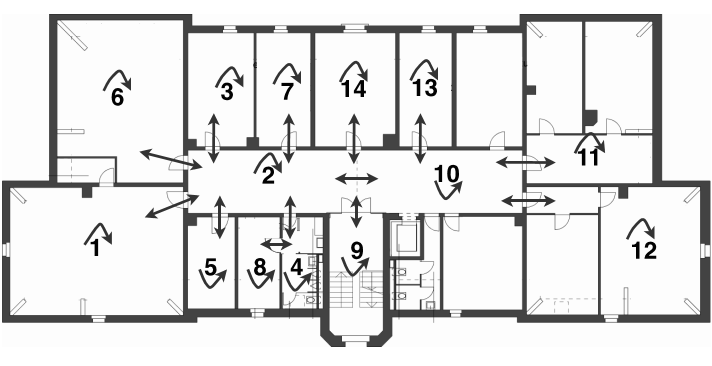
\includegraphics[width=1.0\textwidth]{Figures/zone_definition}
\decoRule
\caption[Zone definition]{Zone definition and transitions between zones}
\label{fig:zone_definition}
\end{figure}

For the testing data the three machine learning algorithms had a correct prediction rate of 80 to 99 percent. 

%-----------------------------------
%	SUBSECTION 2
%-----------------------------------
\subsection{Placement, trajectories and configuration}
We distributed the UWB anchor nodes over several rooms to cover the area of interest homogenously. The exact position is indicated in the floor plan of figure \ref{fig:anchor_position}. Whereas the particle filter updated its state every 700 milliseconds, the IMU sensors were updated every 100 milliseconds. The UWB transmitter of the TAG and the ANs operated in radio mode 2 with a datarate of 850 kbps, they were configured to use channel 4 with a central frequency of 3993.6 MHz and an occupied sprectrum of 1300 MHz. Before starting the experiments, a calibration with 1000 measurements per UWB device was made as described in the beginners guide \cite{Beginnersguide}.

\begin{figure}[th]
\centering
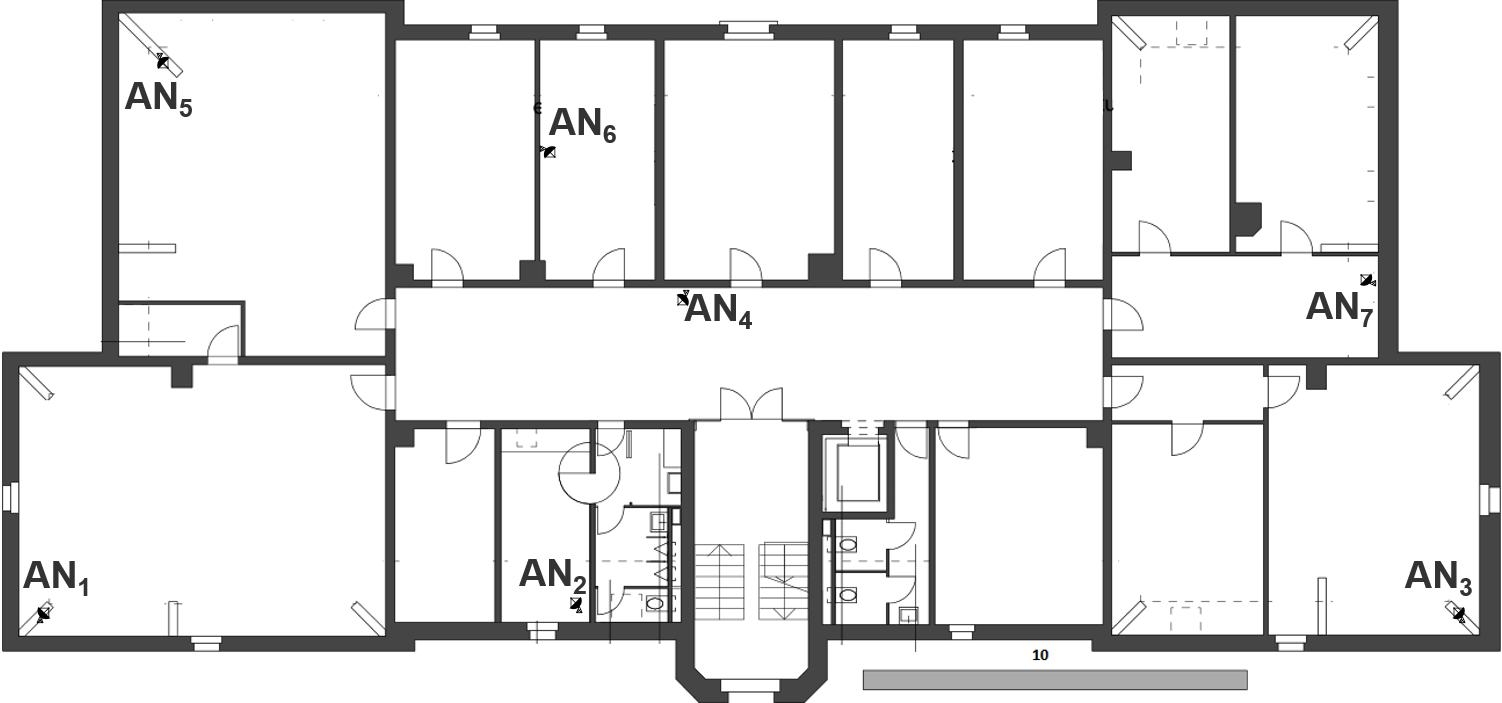
\includegraphics[width=0.8\textwidth]{Figures/anchor_position}
\decoRule
\caption[Anchor node positions]{Distributed anchor nodes on the floor map (with distance reference of 10m).}
\label{fig:anchor_position}
\end{figure}

The TAG was hold in the hand of a pedestrian at the starting point of the trajectories, when the experiments started. The pedestrian walked along the given path indicated in figure \ref{fig:trajectory1}, as soon as he passed a predefined checkpoint the current position estimation was registered. The other three trajectories can be seen in appendix \ref{AppendixA}. Every trajectory was tested with every algorithm at least 5 times.

\begin{figure}[th]
\centering
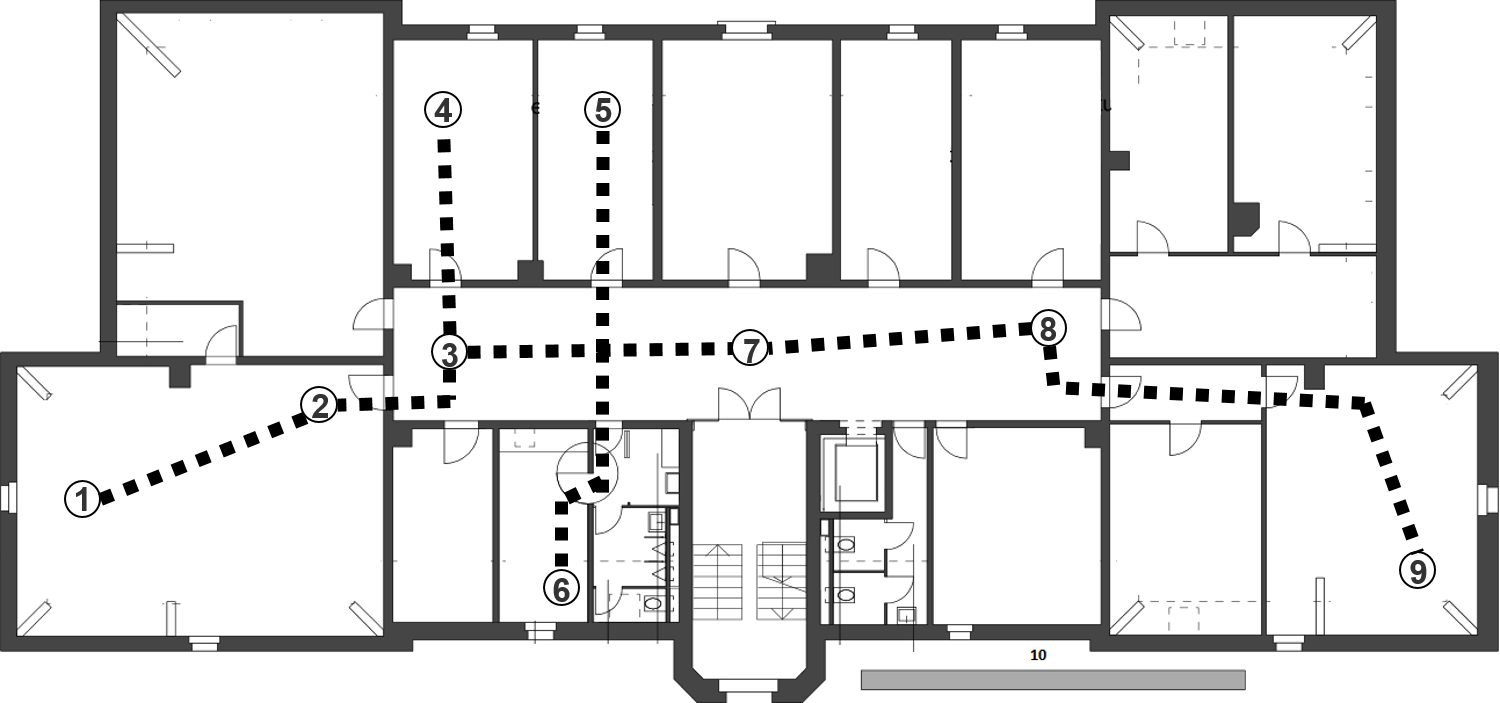
\includegraphics[width=0.8\textwidth]{Figures/trajectory1}
\decoRule
\caption[Trajectory 1]{Trajectory 1 of the four defined trajectories with the position checkpoints.}
\label{fig:trajectory1}
\end{figure}

In an ajusted experiment setup with improved anchor node positions we evaluated a fifth trajectory for every of the three algorithms. We just replaced the AN positions and did not change any other parameter. The new positions of the anchors and the trajectory checkpoints can be seen in figure \ref{fig:trajectory5_withAnchors}. We put the anchor nodes together, such that the distance between the TAG and the farest AN was never more than 20m. Moreover, for a better comparison between the scenarios,  we tried to build a similar distribution of the checkpoints as in the other trajectories. This means we added checkpoints in rooms without an AN and checkpoints at the edges of our test environment. 

\begin{figure}[th]
\centering
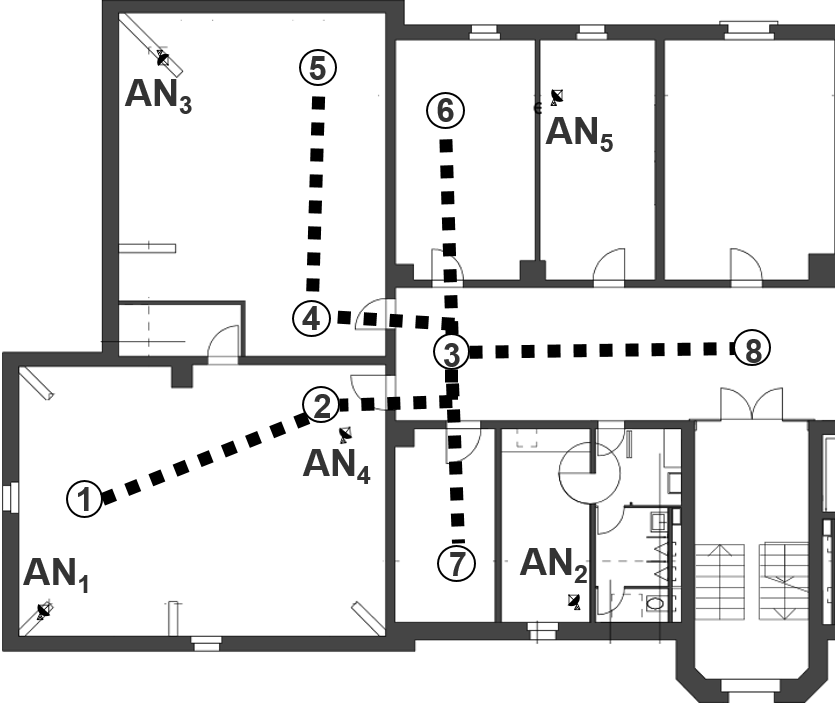
\includegraphics[width=0.5\textwidth]{Figures/trajectory5_withAnchors}
\decoRule
\caption[Trajectory 5]{Trajectory 5 with improved anchor positions.}
\label{fig:trajectory5_withAnchors}
\end{figure}
